A range query is a database operation that retrieves all the records that lies in a range. In this project, we perform range query on 2-dimensional data only. In addition, we only consider a range query where the range is defined as a rectangle. Under these assumptions, a range query can be formalised as a query $\mathcal{Q}(\boldsymbol{l}, \boldsymbol{u})$ where $l,u\in\mathbb{R}^2$.

\begin{mscexample}
	For example, assume we have the points
	$$
	[(1,2), (3,4), (3.5, 4), (5,6)]
	$$
	and the range query $\mathcal{Q}((2,3), (5,5))$, as shown below:
	
	\begin{minipage}[t]{\linewidth}
	\centering
   	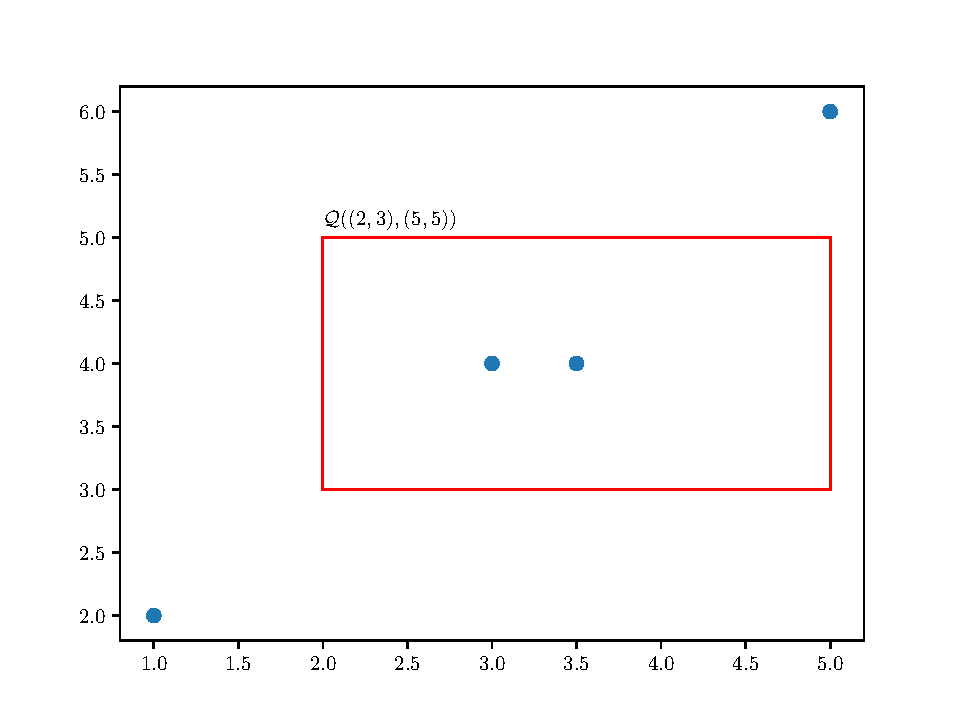
\includegraphics[width=10cm]{graphs/implementation/queries/range_query.pdf}
   	\label{fig:range_query_demo}
   	\captionof{figure}{A Range Query Example where $\mathcal{Q}(\boldsymbol{l}, \boldsymbol{u})=\mathcal{Q}((2,3),(5,5))$}
	\end{minipage}
	
In this example, the range query should return the points that lies inside the red rectangle, i.e. $[(3,4), (3.5, 4)]$.

\end{mscexample}

\subsubsection{Range Query with $K$D-Tree}

% TODO: THIS ALGORITHM IS STILL NOT COMPLETE, and hard to follow.

\begin{figure}[htp]
    \centering
    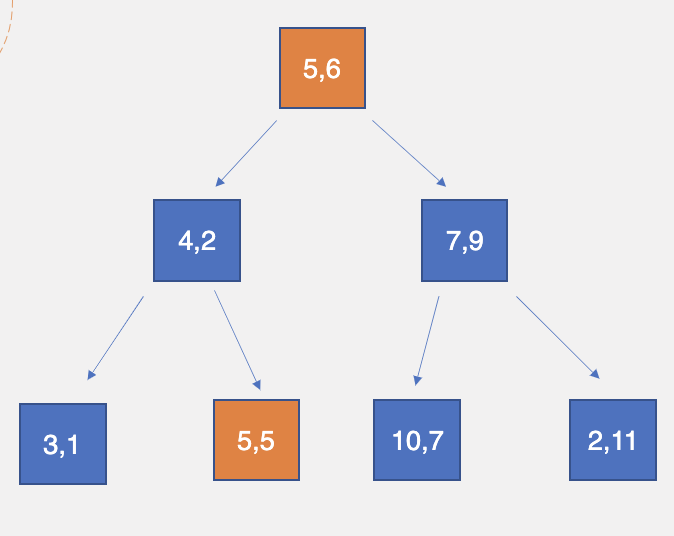
\includegraphics[width=0.4\textwidth]{graphs/Range_Query_Tree.png}
    \caption{$K$D-Tree for Range Query}
    \label{fig:KD-Tree_for_Range Query}
\end{figure}

\begin{figure}[htp]
    \centering
    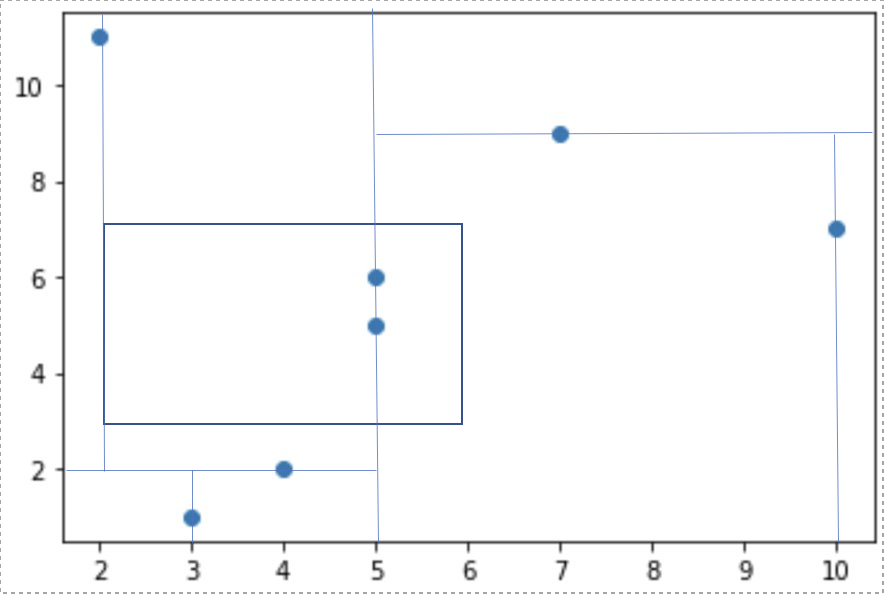
\includegraphics[width=0.6\textwidth]{graphs/Range_Query_plot.png}
    \caption{$K$D-Tree Range Query Plot on 2-dimentional plane}
    \label{fig:KD_Tree_Range_Query_Plot}
\end{figure}


We check the validity of a point lying withing the rectangle by checking the range of x coordinate and y coordinate of a point.

\begin{mscexample}
    For example we have a tree with Point list as 

	$$((5,6),(4,2),(7,9),(3,1),(5,5),(10,7),(2,11))$$
	
	and with lower bound = $(2,3)$ and upper bound = $(6,7)$, we will get a tree as is shown in \ref{fig:KD-Tree_for_Range Query}. We can see the points along with the rectangle range plotted in \ref{fig:KD_Tree_Range_Query_Plot}. Points $(5,5)$ and $(5,6)$ are returned in the query since they lie within the rectangle as seen in the plot. First the root point is checked and since the x-coordinate and y-coordinate both lie within the rectangle bounds i.e., $2$ > $5$ > $6$ and $3$ > $6$ > $7$. It then checks if the x-coordinate is lower than or greater than the lower bound x-coordinate. Since the value is larger than lower bound x-coordinate that is $2$ it will then traverse to the left. In the left it has child node as $(4,2)$ however, since the y-coordinate doesn't lie in the range of the upper bound this point is not selected. Therefore, it recursively traverses the tree and checks if the point lies within the bound until it reaches a leaf.
\end{mscexample}

\subsubsection{Range Query with LISA}

For a range query $\mathcal{Q}(\boldsymbol{l},\boldsymbol{u})$, we first find the cells that overlap with $\mathcal{Q}$. Then we decompose $\mathcal{Q}$ into the union of smaller query rectangles $\bigcup \mathcal{Q}_i$ such that each smaller query rectangles intersects only one cell, as shown in the Fig. \ref{fig:Range_Query_Lisa}.

\begin{figure*}[t]
    \centering
    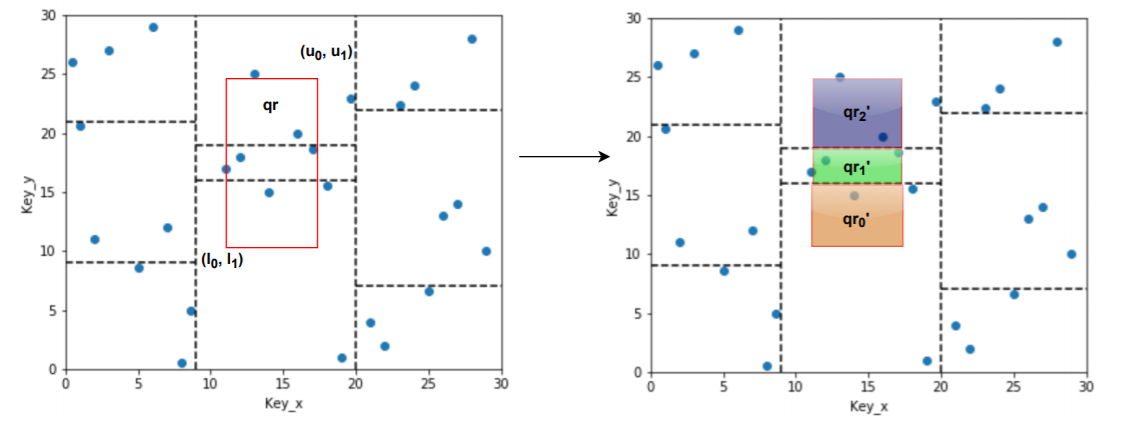
\includegraphics[width=1\textwidth]{graphs/range_query_lisa.png}
    \caption{Range Query Search in Lisa.
    1) Find the cells that overlap with query rectangle qr. \\
    2) Decompose qr into the unions of smaller query rectangles, each of which intersect one only one cell. \\
    3) Find shards corresponding to lower and upper coordinates for each query rectangle, and perform a sequential search. }
    \label{fig:Range_Query_Lisa}
\end{figure*}

 Suppose that $\mathcal{Q}=\bigcup \mathcal{Q}_i$ where $\mathcal{Q}_i=[l_{i_0}, u_{i_o})\times [l_{i_1}, u_{i_1})$, i.e. we have $\mathcal{Q}_i$ representing the $i$th smaller query rectangles of one cell $C_j$.
 
 Then we can calculate the mapped values of $\mathcal{Q}_i$, i.e. $\mathcal{M}(l_{i_0}, l_{i_1})$ and $\mathcal{M}(u_{i_0}, u_{i_1})$. For simplicity, we use $m_l^{(i)}$ and $m_u^{(i)}$ to denote $\mathcal{M}(l_{i_0}, l_{i_1})$ and $\mathcal{M}(u_{i_0}, u_{i_1})$ respectively.
 
After creating corresponding mapped values, we then apply the shard prediction function $\mathcal{SP}(m_{l}^{i})$ and $\mathcal{SP}(m_{u}^{i})$ to predict the shard that could possibly contain keys that lie in the query rectangle $\mathcal{Q}_i$. Then in each shard, we perform a sequential search to find the desired keys. 

